\chapter{Contexte}
    \section{Introduction}
        
    \paragraph{}
    Ce mémoire s'incrit dans le cadre d'une collaboration entre
    l'URGéo et Kay Nou Tek. Ce projet est financé par l’Ambassade
    de Suisse en Haïti et a pour objectif d’explorer le potentiel 
    du numérique pour améliorer les pratiques de construction.
    Le but principal de ce travail est
    d'apporter une solution téchnologique  qui facilitera la 
    gestion des données géotechniques en Haïti.
    \paragraph{}
    Ce document comporte deux grandes parties: une première axée
    sur la théorie, se focalisant sur le contexte et les avantages
    de la réalisation d'un tel projet. La seconde partie est plus pratique
    et combine le travail de l'ingénieur logiciel et des analystes programmeurs responsables
    du projet.
    \begin{figure}
        \centering
        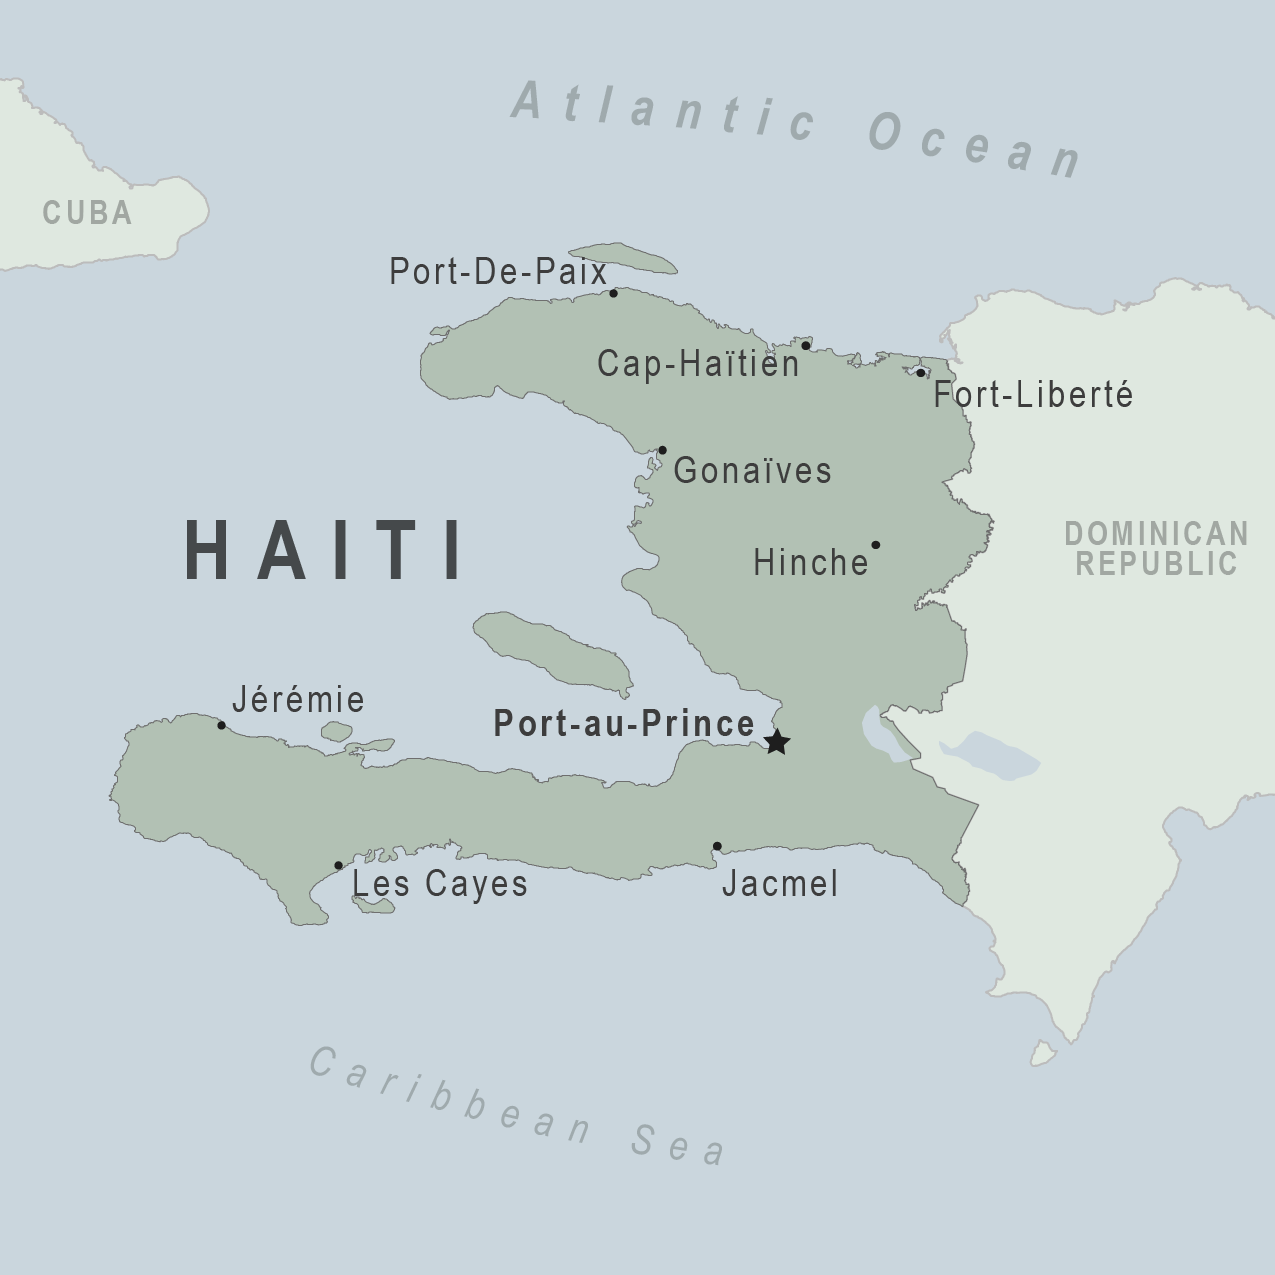
\includegraphics[width=1\textwidth]{images/Contexte/map-haiti.png}
        \caption{Cartographie d'Haïti}
    \end{figure}
        \subsection{Généralités}
            \subsubsection{La géotechique, pourquoi est-ce important ?}
            \par 
La \textbf{géotechnique} est l’ensemble des 
activités liées aux applications de la mécanique des sols, de la mécanique 
des roches et de la géologie de l’ingénieur\footnote{
    Définition selon l’Union syndicale géotechnique accessible via ce lien: 
    \url{http://u-s-g.org/profession-geotechnicien.asp?idpage=1}}.
Au cours d'un projet d'aménagement, dans le but d'assurer  la fiabilité et la durabilité
des ouvrages, le constructeur est dans l'obligation de prendre en compte
la nature du sous-sol du site où il est prévu de construire.

Il s'agit en fait d'adapter le projet au site envisagé.
\par
La mission du géotechnicien consiste principalement à \cite{Chamel}\cite{benachenhou2019approche}:
\begin{itemize}
    \item définir les cadres géologique, hydrogéologique et topographique 
    du site étudié ;
    \item définir les aléas existants vis-à-vis des risques naturels : 
    détection des cavités, stabilité général d’un site (par rapport au 
    glissement de terrain par exemple), sismicité.
    \item définir les terrassements : faisabilité, réemploi des matériaux, 
    tenus des talus et parois des fouilles ;
    \item définir l’influence des circulations d’eaux souterraines, 
    agressivité de l’eau vis-à-vis des bétons ;
    \item définir comment la nature et la répartition des 
    formations géologiques pourrait influencer la réalisation des travaux et la conception 
    de l’ouvrage.
\end{itemize}
\paragraph{}
En général, le géotechnicien résume sa mission dans un rapport.
Ce rapport comprend les résultats des différents tests (Figure \ref{fig:test_penetrometrique}) 
réalisés : essais de pénétration, forages, essais de laboratoire,
essais géophysiques, etc.
\begin{figure}
    \centering
    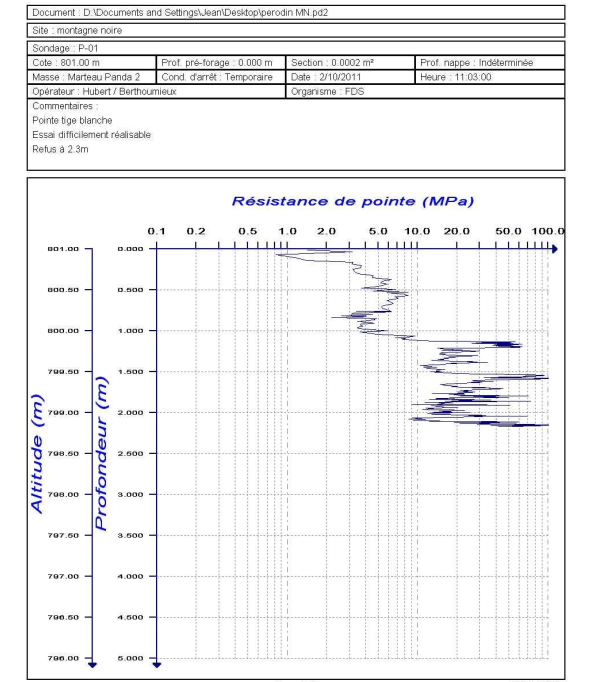
\includegraphics[width=0.5\textwidth]{images/Contexte/penetrographe.png}
    \caption{Exemple de résultat d'un essai pénétrométrique dynamique }\cite{penetrometrie}
    \label{fig:test_penetrometrique}
\end{figure} 

Ce rapport est rédigé non seulement dans le but d’informer le client sur la nature des interventions
, mais aussi d’exposer les principaux résultats des tests recueillis, de façon à mener à bien
l’exécution des projets.
\par
La zone d'étude de ce projet correspond à Haïti (Figure \ref{fig:haiti}).
\begin{figure}
    \centering
    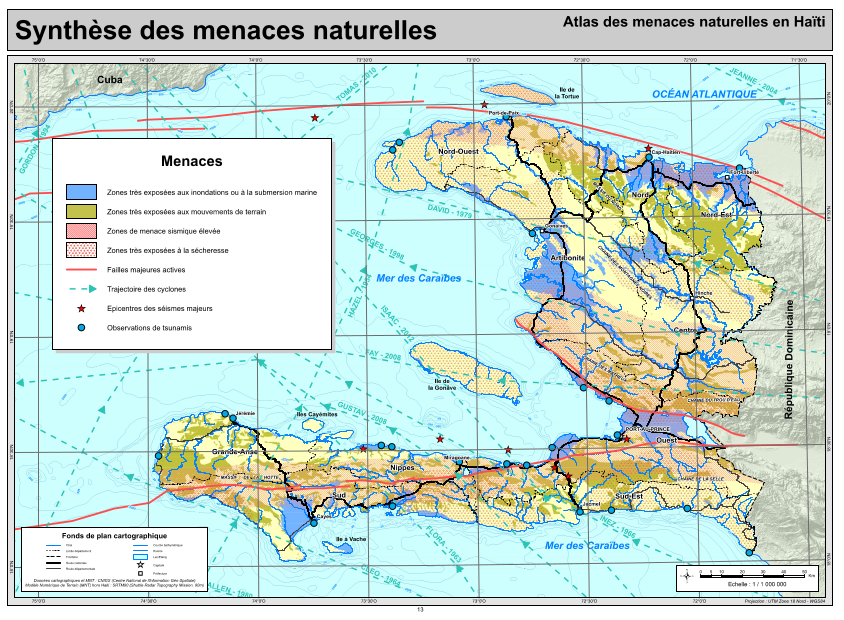
\includegraphics[width=1\textwidth]{images/Contexte/haiti.png}
    \caption{Cartographie d'Haïti, Synthèse des menaces naturelles  \cite{ciat}}
    \label{fig:haiti}
\end{figure}
Ce pays situé dans les Caraïbes a une superficie de  \SI{27750}{\kilo\metre\squared}\cite{superficie}.
L'importance des données géotechniques s'est montrée incontournable dans ce pays particulièrement 
après un séisme dévastateur en Janvier 2010.

\paragraph{}
Vulgairement appelé \textit{Goudougoudou}, un séisme de magnitude 7\cite{mondiale2010haiti} sur l'échelle de Richter, 
a fait de grands ravages sur l'île. Les pertes enregistrées, tant en vies humaines qu'en biens
matériels, ne faisaient que refléter l'ignorance de certains et le laisser-aller des autres. 
Des bâtiments construits défavorablement, des ravines devenues des villages ou simplement des 
constructions effectuées sur un sol inadéquat; telles étaient les causes majeures de ces 
pertes. En Haïti, le plus souvent les constructions sont pris à la légère.
\textit{
    Un recensement national en 2003 a rapporté que 8\% des bâtiments dans les zones urbaines d'Haïti sont
    les bidonvilles (Figure : \ref{fig:bidonville})    
    , connus sous le nom de kay atè, et 78\% des maisons sont 
    des maisons en blocs 
    de béton à un étage ou à plusieurs étages \cite{desroches2011overview}.} 
    \begin{figure}
        \centering
        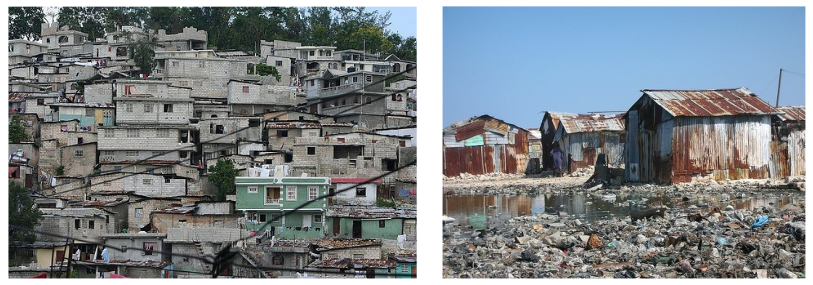
\includegraphics[width=1\textwidth]{images/Contexte/bidonville.png}
        \caption{Bidonvilles aux alentours de Port-au-Prince  \cite{holly1999problemes}}
        \label{fig:bidonville}
    \end{figure}
L' image \ref{fig:musseau} est une représentation typique
 des nombreux exemples de dégâts causés par un glissement de terrain à Musseau en 2008.
 \begin{figure}
    \centering
    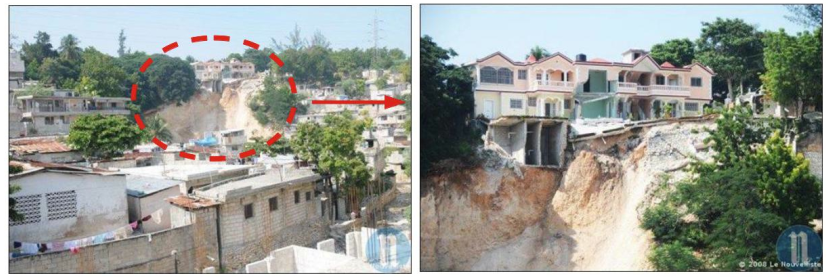
\includegraphics[width=1\textwidth]{images/Contexte/musseau.png}
    \caption{Glissement de terrain à Musseau (photo Le Nouvelliste)}
    \label{fig:musseau}
\end{figure}
\paragraph{}
Le tremblement de terre du 12 Janvier 2010 a ravagé le pays en
tuant plus de 200000 personnes, détruisant
105 000 bâtiments et endommagé 280 000 bâtiments \cite{mondiale2010haiti}.
Ce qui a abouti à près d'un million de sans-abris selon  le journal 
\textit{Natural Hazards and Earth System Sciences Discussions} \cite{daniell2013uncovering}.
Avec une 
étude de sol et des données géotechniques adéquates, un ingénieur pourrait orienter son travail
en connaissance de cause. Par conséquent, depuis maintenant une bonne décennie, les demandes
se multiplient pour l'accès à ces informations.  




            \subsubsection{Production et gestion des données géotechiques en Haïti}
                \par
Les outils papiers utilisés pour le moment sont très vulnérables à des
catastrophes comme des incendies ou des tremblements de terre. La perte 
des documents de référence entraînerait un travail
colossal pour le recouvrement des informations relatives à chaque 
dossier.
\par
Diverses instances détiennent les données recueillies au cours
de leurs études géotechiques respectives. 
Ainsi, lorsqu’un particulier a besoin de faire des études de sols, il 
fait appel à des instances clés capables de les prendre en charge. 
Parmi elles que nous avons pu contacter ou avec lesquels nous avons fait un partenariat, citons :
\begin{itemize}
    \item \textbf{URGéo}
    Unité de Recherche en Géosciences 
    \item \textbf{BME}
    Bureau des Mines et de l’Energie
    \item \textbf{SICOD}
    Société d’Ingénierie Constructions et d’Orientations Diverses
    \item \textbf{LNBTP}
    Laboratoire National Du Bâtiment et des Travaux Publics 
    \item \textbf{Géothechsol}
    \item \textbf{Insolflor}
\end{itemize}   

\par
En général ces entreprises s'impliquent dans la construction et la recherche. 
Leur travail consiste à effectuer une reconnaissance/étude géotechnique des sites .
Depuis plusieurs années ils se sont faits remarqués, notamment dans
l'étude des sols avant la construction de grands bâtiments. Ils sont aussi impliqués
dans la réalisation de ponts et de routes sur le territoire
haitien. 
\paragraph{}
Cepandant un problème persiste: les données recueillies par ces instances
ne sont nullememt en sécurité car elle sont stockées sur papier.
De plus, le minimum qui est numérisé n'est pas intégré dans un environnement 
dédié à cela.
L'analyse des données géotechiques sur toute l'étendue du territoire devient
encore plus difficile car aucune instance ne dispose de l'integralité des tests effectués.
Cela implique une exploitation non optimale de ces données.
\paragraph{Les problèmes actuelles}
\paragraph{}
Le plus grand inconvénient dans la gestion actulles des données géotechiques
en Haïti est la sécurité de ces dernières. 
Cet aspect n'est pas anodin et doit être pris en compte dans la gestion d'un système
d'information.
Actuellement, les critères fondamentaux de la securité des données ne sont nullememt en vigueur en dans le cadre des 
des Systèmes d'Information Géotechniques.
\paragraph{Confidentialité : }
On n'a aucune garantie que seules les personnes autorisées 
aient accès aux données géotechiques. Le fait qu'elles soient
stockées que sur papier auguemente les risques qu'une personnes
n'ayant pas le droit d'accès puisse s'acquérir de ces données.
\paragraph{Intégrité : }
Actuellement personne ne peut
garantir que les données géotechniques que l'on a en notre possession 
sont bien celles que l’on croit. L'intégrité n'est pas assurée car le risque
pour que les données géotechniques soit altérées est trop grand.
\paragraph{Disponibilité :}
C'est l'un des plus grand inconvénient de la gestion actuelle des 
données géotechniques. Trouver une étude qui a été réalisée dans un endroit précis
ou à une date pricise n'est pas évidente. Cela coûte beaucoup de temps et de ressource pour effectuer
les recherche. Par conséquent, le facteur de disponibilité n'est pas 
au rendez-vous car le délai d'acces aux informations est trop long.

\paragraph{}
Divers autres problèmes peuvent être constatés dans la gestion
des données géotechniques en Haïti. Notemment le fait que ces données
ne soient pas à l'abrit des catastrophes humaines (sabotage) et naturelles
(incendies, tremblement de terre, inondation, etc).


\par    
\begin{table}
        \centering
        \begin{tabular}{|p{0.10\linewidth}|p{0.80\linewidth}|}
        \hline
                \textbf{No} & \textbf{Problèmes} \\
                \hline
                    1&
                    Non disponibilité des données
                         \\
                \hline
                2&
                Données susceptibles aux catastrophes humaines et naturelles.
                    \\
                \hline
                3&
                Risques de récidive des réalisations de test
                    \\
                \hline
                4&
                Coûts liés à la gestion archaïque
                    \\
                \hline
                5&
                Risque élevée de la non intégrité
                        \\
                \hline
                6&
                Les données sont eparpillées
                        \\
                \hline
                7&
                Le traitement des données n'est pas évident
                        \\
                \hline
                8&
                Non exploitation des données par les spécialistes et universitaires
                        \\
                \hline 
                9&
                Non exploitation des données par l'état pour les prises de certaines décisions
                        \\
                \hline 
                10&
                Données non sécurisées
                        \\
                \hline 
        \end{tabular}
        \caption{Principaux problèmes liés à la gestion des données géotechniques en Haïti} \label{tab:problemes}
\end{table}
\par
        \subsection{Problématique}
        \textbf{Comment arriver à créer une base de données permettant de 
        présenter et référencer l'ensemble des données géotechniques dans un Systéme
        d’Information Géographique (SIG) ?}
       
        \subsection{Panorama du projet}
            À l'ère où le numérique prend mondialement son expansion, proposer une solution bien plus 
efficace et efficiente se fait grandement ressentir. 
Avant d'entrer d'emblée dans le vif du sujet, nous aborderons 
d'abord l'état de l'art. Cette phase va nous permettre de capitaliser le 
savoir et le savoir-faire existants, et de ne pas refaire des expériences 
qui auraient déjà été faites et dont les conclusions ont déjà été validées 
par des pairs.
\par
Par la suite, on se penchera sur les différents éléments de réponse que l'on 
pourrait apporter au problème confronté.
Enfin nous metterons l'emphase sur l'implémentation des diverses solutions 
que l'on propose.


    \section{Étude de l'existant}
        \subsection{Les BDD géotechniques dans le monde}
            % \paragraph{}
% Un système de gestion des informations géotechiques s'avère incontournable
% dans un environnement de géoscience. Beaucoup d'universités et d'entreprises 
% privées ainsi que l'état dans certains pays à travers le monde se sont déjà 
% penchés sur la question. 
% \paragraph{}
% Les résutats divergent sur quelques détails à propos des technologies utilisées mais 
% l'objectif est généralement le même: 
% constituer une base de données renseignée regroupant tous les points (sondages, essais
% in situ ou en laboratoire) améliorant la connaissance des caractéristiques géomécaniques des
% formations d'une zone.
% Par exemple, dans les Caraïbes, plus précisement sur l'Ile de Cayenne, un tel système a permis
% de mieux appréhender les types de problèmes
% spécifiques au site, et donc de mieux dimensionner les campagnes de reconnaissance
% géotechniques, aussi bien sur le plan technique que financier
% \cite{cayenne}.
% \par 
% L'une des faiblesses de certains projets est l'utilisation des outils de Microsoft
% qui ne semblent pas assez 
% adéquats. Ils sont trop génériques, ce qui empêche un stockage intelligent des données géotechniques
% \cite{antoljak2012subsurface}.

% %......................

% \paragraph{}D'autres se basent de préférence sur la conception d'une architecture d'information 
% géotechnique à l'aide de services Web
% \cite{zimmermann2003design}.
% Cette architecture d'information a été implémentée à Los Angeles afin de permettre les échanges 
% d'informations géotechniques accessibles pour tous. Les avantages apportés par une telle 
% application pourraient tant se sentir pour des études concernant les risques sismiques que pour 
% une meilleure approche lors des estimations effectuées par des compagnies d'assurance. 

% \paragraph{}
% Au Canada, plusieurs projets identiques ont vu le jour, notemment l'élabora\-tion d'une base 
% de données géoscientifiques dans le but d’aider à la finalisation de la 
% cartographie des dépôts en surface et en subsurface
% \cite{russell1996regional}.

% %............................

% \paragraph{}
% En 2011, un séisme a frappé la région de Canterbury (Nouvelle-Zélande). Une base de données en ligne a été développée pour
% la reconstruction de Christchurch à la suite du tremblement de terre:
% La base de données géotechniques de Canterbury (CGD). Elle
% a été conçue comme un référentiel consultable pour le partage d'informations géotechniques existantes et nouvelles
% ainsi que des applications géotechniques de soutien pour les autorisations de construction. En mars
% 2015, la base de données contient plus de 18000 enregistrements d'essais de pénétration de cône, 4000 forages, 1000
% piézomètres accompagnés de registres de surveillance des eaux souterraines, 6000 enregistrements de tests de laboratoire
% plus d'autres données. 

% \par
% Le CGD (Figure: \ref{fig:canterbury}) a été conçu comme un référentiel consultable pour les informations géotechniques existantes et nouvelles
% ainsi que des applications géotechniques de soutien pour les autorisations de construction. Tandis que
% les données sont principalement utilisées pour la conception géotechnique de l'amélioration du sol, la fondation du bâtiment,
% réparations, fondations de nouveaux bâtiments et conception géotechnique pour les réparations d'infrastructures, il peut
% également être utilisé à des fins plus stratégiques tel que l'aide à la récupération pour de futures
% catastrophes naturelles.
% \cite{scott2015benefits}

% \begin{figure}[t]
%     \centering
%     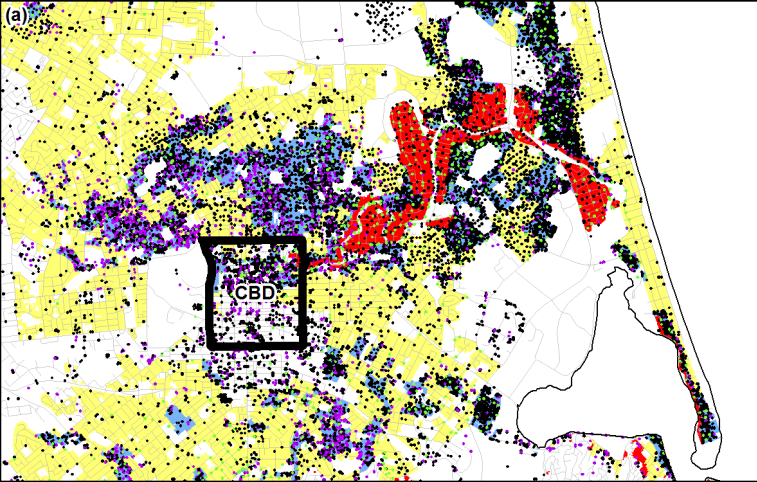
\includegraphics[width=1\textwidth]{images/Contexte/cgd.png}
%     % \caption{Visualisation des résultats de la base de données de Canterbury \cite{scott2015benefits}.}
%     \label{fig:canterbury}
% \end{figure}

% %............................

% \paragraph{}
% L'Afrique ne fait pas exception à la liste des multiples endroits ayant adopté l'idée
% de concevoir des bases de données géotechniques.
% Par exemple, celle de la ville de Tunis (Tunisie) est orientée vers la cartographie géotechnique.
% \par
% Le modèle choisi a permis, après une analyse
% pré1iminaire très importante, une description globale et
% totale de toutes les données géologiques et géotechniques collectées sur le site de Tunis. Il
% assure, de plus, une indépendance physique et logique, un partage des données (une même donnée accessible  
% par plusieurs programmes), une non-redondance des données, une grande facilité des relations
% entre fichiers indépendants, une intégrité (validité)
% totale des données. 
% \textit{S'y ajoutent une souplesse remarquable d'interrogation de TUNIS-DATA-BANK
% assurée par l'emploi d'un langage d'interrogation spécifique et l'utilisation des opérateurs et des connecteurs
% logiques, une automatisation totale des tâches de la
% phase de la manipulation de la base de données et une
% sécurité totale des fichiers.}
% \cite{mongereau1988conception}

% %..................
% \paragraph{} 
% Parmi les BDD géotechniques gouvernementales (Figure:\ref{fig:BDG}), la Base de Données Géotechniques
% (BDG) du gouvernement canadien, plus précisément le
% ministère des transports du Québec, et le "Geotechnical Web Mapping App" (Figure:\ref{fig:wash}) se font remarquer
% de par leur simplicité et leur efficacité. Ces deux systèmes présentent les sondages, les forages ainsi que les 
% propriétés des sols et des roches dans plusieurs zones de ces deux pays.
% Un webmap est utilisé pour faciliter la visualisation de ces données.
% De plus, le résultat de chaque étude est mis à la disposition du public
% via un lien PDF.

% \begin{figure}[t]
%     \centering
%     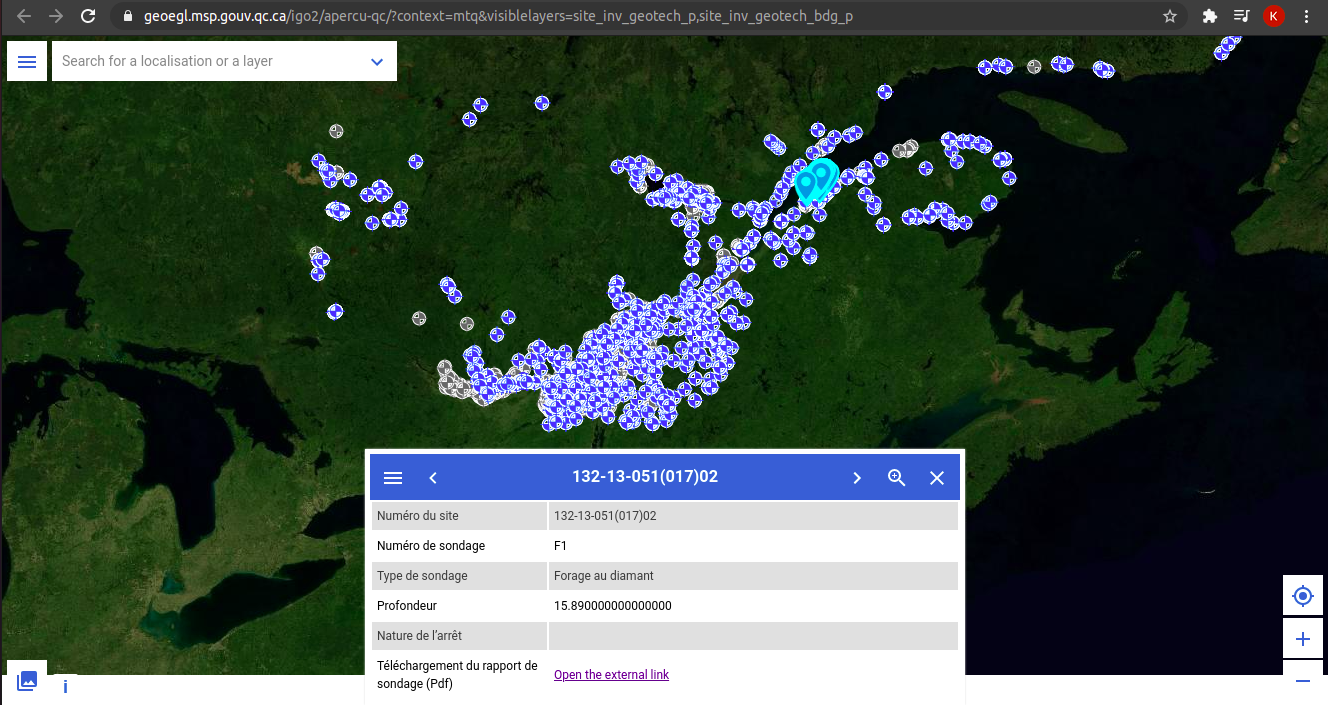
\includegraphics[width=1\textwidth]{images/Contexte/bdg.png}
%     % \caption{Webmap de la BDG du gouvernement du Canada \cite{canadagov}}
%     \label{fig:BDG}
% \end{figure}
% \begin{figure}[t]
%     \centering
%     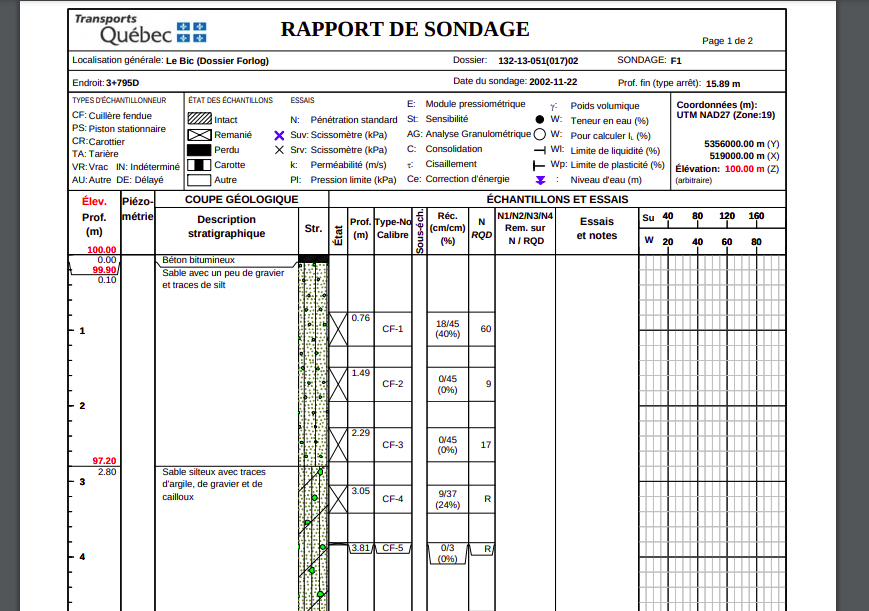
\includegraphics[width=1\textwidth]{images/Contexte/pdf_bdg.png}
%     \caption{PDF d'un rapport de sondage de la BDG du gouvernement du Canada \cite{linkpdfcanada}}
%     \label{fig:PDF_BDG}
% \end{figure}
% \begin{figure}[t]
%     \centering
%     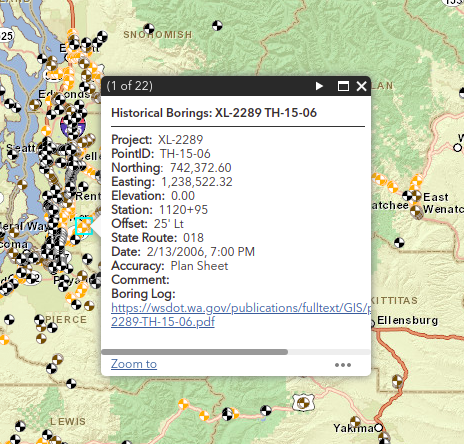
\includegraphics[width=1\textwidth]{images/Contexte/wash.png}
%     \caption{Information sur une étude spécifique dans le Geotechnical Web Mapping App \cite{map1}}
%     \label{fig:wash}
% \end{figure}

% \paragraph{}
% L’implémentation de tous ces SIG par des organismes internationaux résulte à des données considérées 
% comme étant le système d’archivage officiel dans leur domaine de spécialité.
% Le rythme de migration de ces données dans le SIG Web connait une croissance exponentielle. 
% Quelques exemples sont donnés dans le tableau \ref{tab:someBDD}.
% \par
% Avec son mouvement vers le cloud et sur le Web, son intégration à l'information 
% en temps réel via l'Internet des objets, le SIG est devenu une plateforme 
% pertinente pour presque toutes les activités humaines - un système nerveux de 
% la planète. Alors que notre pays est confronté au problèmes de gestion et de vulgarisation 
% des données géotechiques, les SIG joueront un rôle de plus 
% en plus important et 
% fourniront un moyen de communiquer des solutions en utilisant le langage commun de 
% la cartographie.

% \par    
% \begin{table}
%         \centering
%         \begin{tabular}{|p{0.40\linewidth}|p{0.60\linewidth}|}
%         \hline
%                 \textbf{BDD} & \textbf{Fonctions} \\
%                 \hline
%                     British Geological Survey (BGS) créée par le
%                     Royaume-Uni&
%                     Fournisseur de données, 
%                     d’informations et de connaissances 
%                     géoscientifiques objectives britannique
%                          \\
%                 \hline
%                     SERNAGEOMIN (Figure:\ref{fig:chili}) créée par le
%                     Gouvernement du Chili&
%                     Génération 
%                     d'informations géologiques sur le territoire 
%                     chilien, ses dangers géologiques et sa mise 
%                     à disposition des citoyens
%                          \\
%                 \hline 
%                     La base de données géotechniques de Canterbury (CGD) créée par le
%                     Gouvernement de la Nouvelle Zélande&
%                     Génération 
%                     d'informations géologiques sur le territoire 
%                     chilien, ses dangers géologiques et sa mise 
%                     à disposition des citoyens
%                         \\
%                 \hline 
%                     DBG créée par
%                     Ministère des transports du Québec&
%                     - Présentaion des sondages
%                     - Présentaion des forages sous forme schématique
%                     - Présentaion des propriétés des sols et des roches
%                     - Présentaion de la qualité de l’eau souterraine
%                         \\
%                 \hline 
%                 GISOS créée par
%                 trois organismes: BRGM, INERIS, INPL-LAEGO&
%                     - Accès facile aux informations sur les forages
%                     - Accès aux mouvements de terrain
%                     - Accès aux mesures topographiques
%                     - Accès aux essais au laboratoire
%                         \\
%                 \hline 
%                 Base de données géotechniques, géodésiques
%                  et géophysiques dans les argiles du Trièves créée par
%                  le conseil général de l'Isère&
%                         -Mise à disposition des utilisateurs potentiels, scientifiques ou opérationnels des informations
%                         géotechniques, géodésiques et géophysiques.
%                        \\
%                 \hline 
%                 SIGPEG
%                 et géophysiques dans les argiles du Trièves&
%                         - Accès aux informations sur les données
%                         cartographiques, géophysiques, géotechniques, sur les puits forés
%                             \\
%                 \hline 
%         \end{tabular}
%         \caption{Présentation de quelques BDD géotechniques dans le monde} \label{tab:someBDD}
% \end{table}
% \par

% \begin{figure}[t]
%     \centering
%     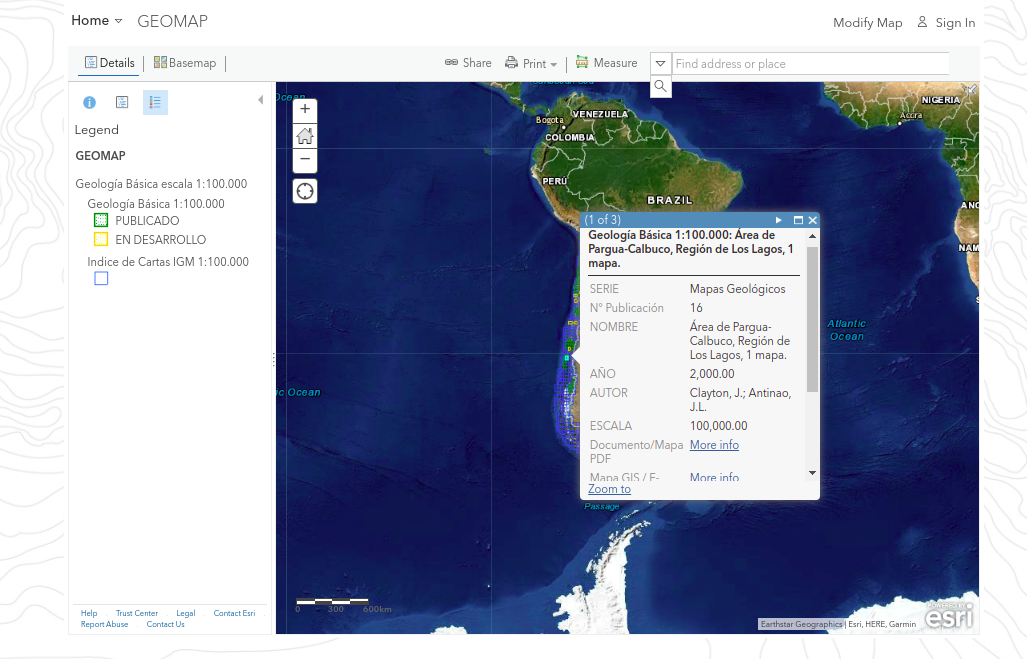
\includegraphics[width=1\textwidth]{images/Contexte/chili.png}
%     \caption{Webmap de SERNAGEOMIN \cite{map2}}
%     \label{fig:chili}
% \end{figure}

        \subsection{Avantages d'un Système de gestion des Informations Géotechniques}
            \paragraph{}
Les avantages apportés par le développement d'un systeme d'information géotechique
sont multiples.
L'un des plus important est la facilité avec laquelle les données 
peuvent être visualisées, filtrées et manipulées.
De plus, le risque de trouver  des informations inexactes est considérablement
réduite grâce aux protrocoles du métier, à la validation des données et aux processus
de contrôle approfondis.

\textit{ Une 
étude réalisée par Goldin et al.,
(2008) a montré qu'en moyenne 1,24\% des entrées de données dans Excel 
sont saisies de manière incorrecte; l'erreur alors
composés chaque fois que les données sont réintroduites. La mise en place 
«à entrée unique» d’une base de données bien conçue réduit les erreurs de 
transcription humaine, source majeure d’inexactitude pour les entreprises
traitant de grandes quantités de données géotechniques.}
\cite{keen2015development}
\paragraph{}
Ce projet peut aussi être
conçu comme un référentiel consultable pour le partage d'informations 
géotechniques existantes et nouvelles.
Il sera un outil de soutien pour les autorisations de construction délivré par l'État haïtien.
\paragraph{}
\par
Ces données peuvent également être utilisées à des fins plus stratégiques telles que l'aide à la
relèvement en cas de futures catastrophes naturelles.
Elles peuvent être utiles pour  l'élaboration des processus réglementaires.
La vaste base de données géotechniques
combinée à d'autres ensembles de données permettra un examen et une modélisation approfondis du terrain
et la performance de l'infrastructure à construire. 
\par
Les leçons tirées de ces analyses peuvent être appliquées pour
améliorer la résilience et également utilisé pour éclairer les 
décisions de politique réglementaire dans d'autres domaines en Haïti.
\paragraph{}
En plus du partage des données, une base de données géotechniques
offre les avantages suivants:
\begin{itemize}
    \item Diminution des coûts de maintenance des données géotechiques
    \item Les professionels peuvent accéder plus facilement aux informations géotechniques
    fournis par d'autres, économisant certains frais d'enquête
    \item Des évaluations de haut niveau peuvent être effectuées pour des
    projets utilisant des informations de la zone environnante pour
    mieux renseigner le profil géotechnique avant de s'engager à
    études plus détaillées
    \item Les données d'une zone peuvent être
    accessible pour servir de référence pour le terrain  dans des contextes géologiques similaires
    \item Les fournisseurs d'infrastructure peuvent être mieux informés
    et mieux cibler les zones les plus vulnérables , et, suite à un événement, optimiser les réparations
    \item  Les données souterraines peuvent être fournies aux autorités réglementaires
    et les décideurs pour leur permettre de prendre
    les décisions d'aménagement du territoire et déterminer la pertinence
    des stratégies et solutions d'investissement
    \item  Les entrepreneurs spécialisés peuvent évaluer les opportunités
    investir dans des équipements spécialisés et améliorer les sols de construction
    \item Améliorer la modélisation de sinistres catastrophes pour les assurances et
    la gestion des dangers. Cela facilerait la réalisation de scénario approprié
\end{itemize}

\paragraph{}
Cette base de données géotechiques permet aussi à la communauté
scientifique d'avoir accès à certaines données qui normalement seraient 
hosrs de porté cause des contraintes budgétaires. La recherche devient alors plus 
facile dans le domaine de la géotechique en Haïti.


\paragraph{}
Étant donné que cet outil n'existe pas encore
en Haïti, l'ampleur de ce projet fait donc surface.
D'où l'implémentation qui suit.


\par    
\begin{table}
        \centering
        \begin{tabular}{|p{0.10\linewidth}|p{0.80\linewidth}|}
        \hline
                \textbf{ } & \textbf{Avantages} \\
                \hline
                    1 &
                    Réduction du risque de trouver des informations inexactes
                    \\
                \hline 
                    2 &
                    Pas de duplication des données
                    \\
                \hline 
                    3 &
                    Création d'un référentiel consultable pour le partage d’informations géotechniques
                    \\
                \hline 
                    4 &
                    Diminution des coûts de maintenance des données géotechiques
                    \\
                \hline 
                    5 &
                    Disponibilité des données géotechiques
                    \\
                \hline 
                    6 &
                    Sécurité des données géotechiques
                    \\
                \hline 
                    7 &
                    Faciliter les prises de décisions d’aménagement du territoire 
                    et déterminer la pertinence des stratégies et solutions d’investissement
                    \\
                \hline 
                    8 &
                    Améliorer la modélisation de sinistres catastrophes pour les assurances
                    \\
            \hline 
        \end{tabular}
        \caption{Listes de quelques avantages d'une base de données géotechniques} \label{tab:avantages}
\end{table}
\par

    \section{La solution proposée}
        \paragraph{}
        Face aux différents problèmes que l'on constate, la solution que l'on propose est la suivante:
        Il s'agit de créer une base de données permettant de présenter et référencer l’ensemble des 
        données géotechniques dans un Système d’Information Géographique.
    
        \subsection{Les apports de cette solution}
            Ce sera une base de données relationnelle liée a une application web
            \footnote{Le choix des technologies est justifié dans le chapitre 3} 
            qui va assurer:
            \begin{itemize}
                \item la disponibilité des données
                \item l'intégrité des données
                \item la confidentialité
                \item la non répudiation
                \item un filtrage optimal des données
                \item la visualisation des données via un webmap
                \item l'accès aux données par les professionnels et universitaires
                \item la diminution des coûts liés a la gestion des données
                \item la sécurité des données face aux catastrophes humaines (sabotage)
                \item la sécurité des données face aux catastrophes naturelles (incendie, tremblement de terre, etc)
                \item l'exploitation des données par des entreprises et l'État pour les prises de décisions
                \item l'amélioration des modèles liés aux domaines géotechniques
                \item facilitation des recherches académiques et scientifique dans le domaine géotechique
                \item ...
            \end{itemize}
        \subsection{Analyse des risques}
        Les risques liés à la réalisation de ce projet sont multiples.
        \paragraph{Risques sur le plan social :}
        \begin{itemize}
            \item \textbf{Les entreprises :}
            L'enjeu pricipal est de convaincre les entreprises à accepter de rendre publiques des 
            données qui non seulement ont toujours été privées mais aussi qui coûtent chers. 
            Qu'auront-il à gagner en faisant ce geste ? 
            Comment arriver à les motiver à faire un tel sacrifice ?
            \item \textbf{Les visiteurs :}
            De plus il faut arriver à inciter les professionels et les etudiants à
            visiter la plateforme. Un flux d'activités important montrera l'intéret accordé à l'outil.
        \end{itemize}
        
        \paragraph{Solution :}
        La motivation des entreprises sera issue des avantages que l'on leur offrira et de l'ambiance
        scientique dans laquelle ils se trouveront en utilisant l'outil. 
        Tout un concepte sera mis en oeuvre : celui  \textbf{de science participative}.
        Il s'agit de créer une communauté dans laquelle chacun est libre d'aporter sa contribution 
        à la réussite du projet. Les entreprises seront en symbiose au gré des ingénieurs, étudiants 
        et autres entreprises(banques, assurances, l'État, ...) en quête de données géotechniques.
        Ce sera un environnment de partage entre scientifiques. Une campagne de sensibilisation à l'utilisation 
        de l'outil est prévue. Son importance est capitale dans le processus de motivation dans laquelle 
        tout entrepriseet tout utilisateur doit se retrouver.
        \par
        Pour l'ingénieur, ce sera un outil d'aide à la décision. Il peut optimiser son travail en exploitant
        les données de la plateforme. Ainsi, cela évitra aux particuliers désirant réaliser une construction
        d'être soumis aux lourdes contraintes budgétaires qu'implique une étude de sol.
        \par
        Pour l'étudiant, ce sera un outil de travail lui permettant de s'exercer avec des données réelles 
        et le préparant pour la vie profosionnelle qui l'attend.
        \par
        Pour l'entreprise, ce sera un outil lui permettant d'evaluer les risques d'un investissement. Par 
        exemple une banque peut s'appuyer sur ces données pour savoir si un prêt pour une construction dans une zone
        est risqué ou pas.

        \paragraph{Risques sur le plan technique :}
        \begin{itemize}
            \item \textbf{Réalisation d'un système trop encombrant :}
            Un utilisateur peut se perdre facilement dans un système encombrant. Il convient de le mettre dans un environnment
            pour il pourra facilement naviguer. L'expérience utilisateur (UX) est un point essentiel sur lequel on doit s'attarder.
            \item \textbf{Ne pas utiliser les technologies appropriées :}
            L'analyse des besoins et l'étude de la faisabilité conduisent au choix des téchnologies adéquates pour la réalisation
            du système. Ces choix seront justifiées et adaptés à l'outil. 
            Il s'agit aussi de ne pas réinventer la roue mais de tirer avantage de l'existant tout en réalisant 
            un système adapté à Haïti.
        \end{itemize}
        \paragraph{Solution}
        Le processus UX est global, il ne s’agit pas d’une compétence isolée mais d’une nouvelle 
        démarche qui intègre un nouveau membre de l’équipe projet : l’utilisateur. \cite{Schaudel2020}
        Il s'agira de co-construire l'interface avec l'utilisateur. On lui offre d'abord un espace simple et attrant
        tout en étant à l'écoute de ses feedbacks. Dans ce sens, une version Beta de l'application sera lancé et sera prête
        à être améliorée en fonction des demandes des utilisateurs.
        \par


    \section{Cheminement de la solution}
        \subsection{Implémentation d'une BDD géotechniques}
            \subsubsection{Numérisation des données}
                \par
Au cours de la première étape, des données seront recueillies à 
travers diverses instances, principalement l'URGéo ainsi que d'autres partenaires. 
Enregistrées sous divers formats(papiers, CSV, PDF entre autres), 
ces données seront par la suite normalisées puis numérisées. En 
effet, une structure uniforme devra être imposée afin de satisfaire la 
compréhension de tout particulier et le partage de ces données.
Cette étape a rapport à la standardisation des données et aux protocoles adoptés.
            \subsubsection{Intégration de ces données dans une BDD}
                \par
Évidemment, une simple numérisation ne changerait point grand chose 
si les données restent stockées sur des disques comme à l'ancienne. Ainsi, 
la normalisation ayant apporté un standard et une uniformité au sein des informations 
enregistrées, ces dernières pourront parfaitement être intégrées dans 
une base de données créée à cette fin. Une fois implémentée, cette 
base pourra héberger toutes les informations géotechniques relatives 
à une analyse effectuée par l'une des instances concernées. Plus 
explicitement, l'URGéo pourra enregistrer les résultats obtenus lors 
d'un forage, en alimentant la BDD tout en respectant les critères de 
standardisation.
\paragraph{}
Bien qu'efficace, cette BDD géotechniques reste un concept assez 
abstrait pour un concerné direct qui ne verra aucune différence 
entre ce nouveau format et les fichiers auxquels il était 
précédemment habitué.
        \subsection{Utilisation d'un SIG}
            \subsubsection{Connection de la carte d'Haïti et de la BDD}
                \par
Comme réalisé dans différents pays à travers le monde, la prochaine 
étape consistera à utiliser un Système d'Information Géographique (SIG) 
capable de faciliter l'interprétation scientifique de ces données. 
Les SIG permettent aux utilisateurs de créer leurs propres couches de cartes 
afin de résoudre des problèmes concrets. Ils ont également évolué ces dernières années pour 
devenir un moyen de partage de données et de collaboration, inspirant une 
vision qui devient aujourd’hui une réalité. Une base de données qui 
couvre pratiquement tous les sujets; dans le cas présent, ce sera la géotechnique. 
Une fois le SIG lié à la base, tout intéressé pourra accéder aux informations 
enregistrées, dans un format plus conventionnel. Cela facilitera la visualisation des données. 
Dans le cadre de ce projet, il 
pourra trouver les résultats des tests effectuées au niveau d'une zone précise.
            \subsubsection{Utilisation de fonds de carte}
                \par
Une fois les informations accessibles, l'interprétation devient 
plus évidente; ce qui peut, pourtant, s'avérer insuffisant. Par 
ailleurs, des images relatives au contexte recherché par le scientifique 
le mettra dans un environnement avec le maximum de détails. De ce fait, 
différents fonds de carte seront mis 
à la disposition de ce dernier, facilitant sa manipulation des données. 
L'ingénieur civil voulant faire des études en hydraulique pourra ainsi 
interprêter les données relatives à son domaine en sélectionnant 
le fond le carte qui lui convient.
\paragraph{}
Désormais, tout particulier pourra accéder aux données de la BDD 
géotechnique en se référant à son domaine d'étude. Néanmoins, jusque-là,
l'accès direct aux données de la base demandera l'intervention d'un 
expert en base de données.
        \subsection{Visualisation des données} 
            \subsubsection{Implémentation d'un UI intégrant un webmap}
                \par
Finalement, la dernière étape consistera à mettre à la disposition 
de nos utilisateurs finaux un interface adéquat et facilement 
accessible, leur permettant ainsi d'interagir avec la BDD. Grâce 
à cela, un administrateur pourra directement ajouter, afficher, modifier ou supprimer 
des informations sans avoir à contacter un expert en informatique.
Quant aux simples visiteurs, ils auront la possibilité de visualiter les données sur une carte. 
Ces données vont permettre aux utilisateurs(ingénieurs, étudiants, etc) de prendre des décisions, 
d’analyser des situations précises, ou encore de donner des alertes par rapport à des évènements précis.
\par
En effet, l'autonomie de tous les utilisateurs sans formation préliminaire 
traduira la performance de l'application. L'expérience utilisateur n'est pas anodin dans 
le développement d'un tel système.
            \subsubsection{Publication de l'interface}
                \par
Quelle serait l'utilité d'une application de cette envergure 
si sa portabilité n'était pas prise en compte ? - Aucune. Par 
conséquent, son déploiement dans le cloud relèvera d'un processus incontournable 
afin de la mettre à la disposition de tous les intéressés. Désormais, 
n'importe qui aura la possibilité d'accéder au portail web sans 
installation préalable. Néanmoins, pour une question de sécurité, 
certaines fonctionnalités exigeront à l'utilisateur/administrateur une authentification.
        \begin{figure}[t]
            \centering
            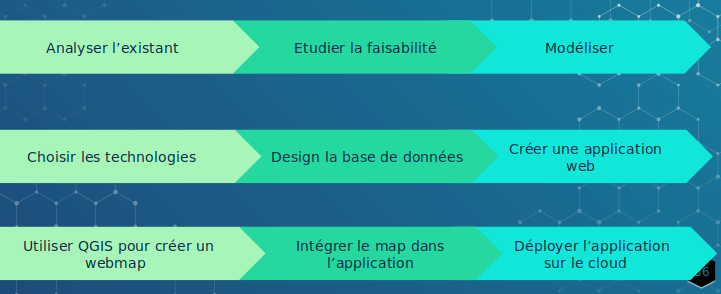
\includegraphics[width=1\textwidth]{images/Contexte/evolution_projetGIS.png}
            \caption{Cheminement de la solution}
        \end{figure}

    \section{Perspective de réalisation}
        \par
Étant plus que pragmatiques, nous ne nous limiterons pas à proposer 
uniquement une solution théorique. Nous mettrons la main à la pâte afin
de donner des résultats palpables et fonctionnels.
\par
Pour ce faire, nous définissons un cheminement, un ensemble d'étapes à 
respecter pour aboutir à un résultat optimal au moindre coût.
Ce cursus comprend cinq grandes étapes: 

\begin{itemize}
    \item \textbf{L'initialisation du projet: }
    Cette étape marque le début de notre long parcours et aura comme principaux
    objets la prise de connaissance du problème (dans le CDC) et l'identification des voeux
    l'URGéo.
    \item \textbf{Planification: }
    Tout grand projet digne de ce nom doit être planifié. C'est au cours de cette étape
    que l'état de l'art sera traité pour prendre connaissance de l'existant et s'inspirer des travaux
    similaires déjà réalisés. Puis vient la phase de l'analyse, de l'évaluation des coûts du projet, 
    du choix  de l'architecture, des modèles,
    ainsi des technologies et des méthodes que l'on aura à utiliser.
    \item \textbf{Exécution: }
    L'essence de cette étape se trouve dans la réalisation même du projet, que ce soit en matière de base de 
    données ou de programmation.
    \item \textbf{Monitoring et contrôle: }
    Ici il s'agit d'effectuer des tests sur la qualité du produit final et et de vérifier si on a atteint le 
    résultat escompté. Notons que cette partie pourra se faire en parallèle avec l'éxécution, en faisant de 
    l'intégration continue.
    \item \textbf{Fermeture: }
    Enfin, on aboutit à la clôture du projet apres déploiement et une potentielle période de maintenance.


\end{itemize}   